\newcommand{\fgLabelledCycle}[1]{
\begin{tikzpicture}
\def \n {#1}
\def \r {2cm}
\def \sp {14}
\def \tt {360/\n}

\foreach \s in {0,...,\numexpr#1-1\relax}
{
\node[draw, circle] at ({\tt * \s}:\r) {$[\s]$};
\draw[->, >=latex] ({\tt * \s + \sp}:\r)
arc ({\tt * \s + \sp}:{\tt * (\s + 1) - \sp}:\r);
}
\end{tikzpicture}}

\newcommand{\fgClock}{
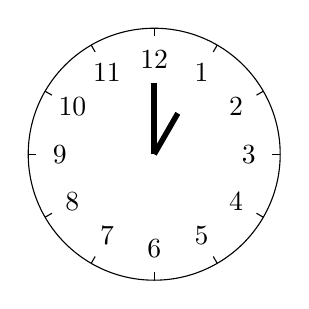
\begin{tikzpicture}
% draw clock border
\draw (0,0) circle [radius=1.6cm];

% draw clock label
\foreach \angle [count=\i] in {60,30,...,-270}
{
\draw (\angle:1.5cm) -- (\angle:1.6cm);
\node at (\angle:1.2cm) {\i};
}

% draw hands
\draw[line width=2pt] (60:0) -- (60:0.6cm);
\draw[line width=2pt] (90:0) -- (90:0.9cm);
\end{tikzpicture}}

\newcommand{\fgNumberLine}[2]{
\begin{tikzpicture}
\foreach \x in {#1,...,#2}
{
\draw (\x, -0.1) -- (\x, 0.1);
\node at (\x, -0.4) {$\x$};
}
\draw (#1, 0) -- (#2, 0);

% bold line at zero
\draw[line width=2pt] (0, -0.15) -- (0, 0.15);
\end{tikzpicture}}

\newcommand{\fgLineSegment}{
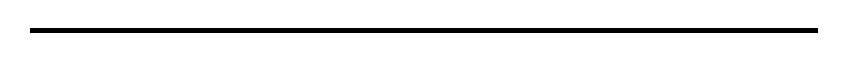
\begin{tikzpicture}
\draw[line width=2pt] (-5, 0) -- (5, 0);
\end{tikzpicture}}

\newcommand{\fgLine}{
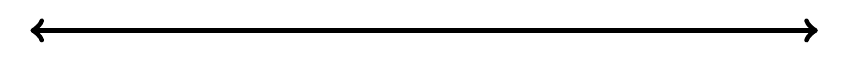
\begin{tikzpicture}
\draw[->, =>latex, line width=2pt] (0, 0) -- (5, 0);
\draw[->, =>latex, line width=2pt] (0, 0) -- (-5, 0);
\end{tikzpicture}}

\newcommand{\fgRay}{
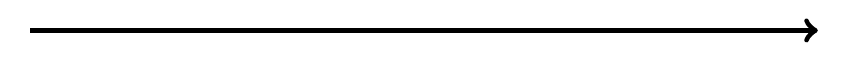
\begin{tikzpicture}
\draw[->, =>latex, line width=2pt] (-5, 0) -- (5, 0);
\end{tikzpicture}}

\newcommand{\fgTwoRays}{
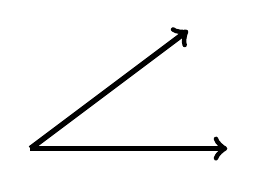
\begin{tikzpicture}
\draw[->, =>latex, line width=2pt] (0, 0) -- (2.5, 0);
\draw[->, =>latex, line width=2pt] (0, 0) -- (2, 1.5);
\end{tikzpicture}}

\newcommand{\fgTwoRaysFar}{
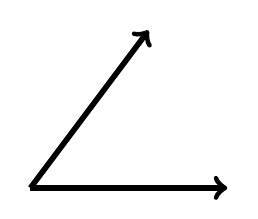
\begin{tikzpicture}
\draw[->, =>latex, line width=2pt] (0, 0) -- (2.5, 0);
\draw[->, =>latex, line width=2pt] (0, 0) -- (1.5, 2);
\end{tikzpicture}}

\newcommand{\fgTwoRaysRight}{
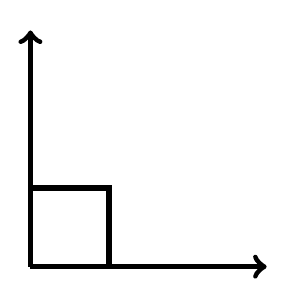
\begin{tikzpicture}
\draw[->, =>latex, line width=2pt] (0, 0) -- (3, 0);
\draw[->, =>latex, line width=2pt] (0, 0) -- (0, 3);
\draw[line width=2pt] (0, 1) -- (1, 1) -- (1, 0);
\end{tikzpicture}}

\newcommand{\fgAsterisk}{
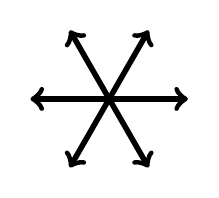
\begin{tikzpicture}
\draw[->, =>latex, line width=2pt] (0, 0) -- (1, 0);
\draw[->, =>latex, line width=2pt] (0, 0) -- (0.5, 0.87);
\draw[->, =>latex, line width=2pt] (0, 0) -- (-0.5, 0.87);
\draw[->, =>latex, line width=2pt] (0, 0) -- (-1, 0);
\draw[->, =>latex, line width=2pt] (0, 0) -- (-0.5, -0.87);
\draw[->, =>latex, line width=2pt] (0, 0) -- (0.5, -0.87);
\end{tikzpicture}}

\newcommand{\fgAngleN}[1]{
\begin{tikzpicture}
\coordinate (A) at (0,0);
\coordinate (B) at (0:3);
\coordinate (C) at (#1:3);
\draw[->, =>latex, line width=2pt] (A) -- (B);
\draw[->, =>latex, line width=2pt] (A) -- (C);
\pic [draw, line width=2pt, "{\small\SI{#1}{\degree}}", angle radius=1.5cm] {angle = B--A--C};
%\draw[line width=2pt] ++(#1:1) arc (#1:0:1) node[midway] ;
\end{tikzpicture}}
